\chapter{Pengujian Implementasi}
\label{apx:implementation-test}

\section{\textit{Unit Test} dan \textit{Integration Test}}

\textit{Integration test} dilakukan selama proses implementasi untuk menguji dan melakukan validasi terhadap fungsionalitas tertentu, termasuk interaksinya dengan instans \textit{dependency} seperti PostgreSQL atau pun Redis. Tidak semua layer abstraksi di bawahnya diuji dengan pengujian yang lebih kecil, seperti \textit{unit testing}. Sebagai contoh, \textit{unit testing} kode repository yang berisi kueri pada basis data tidak akan berguna apabila pengujian dilakukan pada \textit{mock database} alih-alih instans basis data sesungguhnya dengan skema dan data tertentu.

Meskipun begitu, terdapat \textit{unit test} untuk komponen-komponen yang tidak memiliki ketergantungan terhadap instans lain, seperti \textit{unit testing} untuk \textit{early dropper}, pembangkit ID, dan lain-lain.

Total cakupan kode pengujian dari gabungan kedua pengujian adalah 36.1\%. Angka ini sangat kecil, tetapi dapat diprediksi karena hal-hal berikut:

\begin{enumerate}
    \item Angka tersebut juga menghitung kode HTTP server yang tidak diuji pada pengujian terintegrasi. Aplikasi secara keseluruhan akan diuji pada kluster lokal Kubernetes.
    \item Sisa kode yang tidak termasuk code coverage merupakan penanganan kesalahan yang tidak realistis untuk terjadi, sehingga skenario tersebut tidak diuji sama sekali.
\end{enumerate}

Cakupan tersebut memang tidak memuaskan, tetapi memenuhi kebutuhan untuk melakukan validasi atas kebenaran implementasi fitur-fitur penting. Meskipun begitu, cakupan kode pengujian untuk kode proses bisnis jauh lebih tinggi dibandingkan dengan cakupan keseluruhan sebagaimana ditunjukkan pada Gambar \ref{fig:code-coverage}.

\begin{figure}[H]
    \centering
    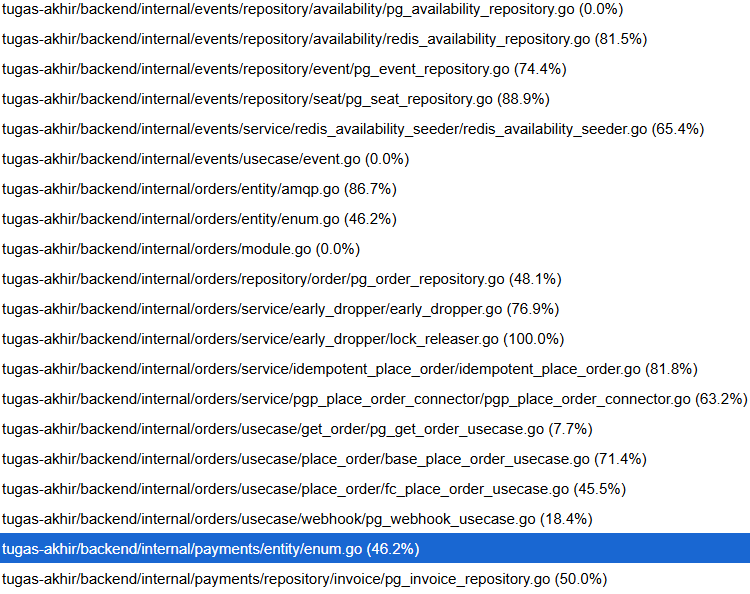
\includegraphics[width=0.7\textwidth]{resources/appendix/coverage.png}
    \caption{Sampel Cakupan Kode Pengujian}
    \label{fig:code-coverage}
\end{figure}

\pagebreak

\section{Kubernetes Lokal}

Pengembangan dan pengujian pada kluster kubernetes lokal dilakukan dengan menggunakan K3d yang mengabstraksikan instans K3s pada Docker. Kakas ini memungkinkan dijalankannya beberapa kluster K3s baik itu satu atau lebih node pada komputer lokal. Satu control plane dan satu agent digunakan untuk kluster backend. Satu control plane lagi digunakan untuk kluster agen penguji.

Pendekatan ini memiliki berbagai keuntungan, yaitu:

\begin{enumerate}
    \item Meminimalkan perbedaan konfigurasi kluster Kubernetes di lokal dan di lingkungan pengujian yang sesungguhnya.
    \item Kebanyakan konfigurasi dapat dibuat pada kluster lokal, sehingga meminimalkan biaya yang harus dikeluarkan untuk pengembangan dan pengujian.
    \item Validasi kebenaran aplikasi, konfigurasi deployment, dan konfigurasi monitoring dengan \textit{end-to-end testing}. \textit{Smoke test} juga dilakukan dengan 200 VU selama 10 menit pada kluster lokal.
\end{enumerate}
